%% GPs for classification and ordinal regression
\lecture{GPs for classification and ordinal regression}{Classification}

\begin{frame}
	\frametitle{GPs for Classification and ordinal regression}
	\begin{itemize}
		\item What if our observation model is non-Gaussian?
		\begin{itemize}
			\item Classification:
			\[
				P(y_n=1|f_n) = \int_{-\infty}^{f_n} {\cal N}(z|0,1)~dz = \phi(f_n)
			\]
			\item Logistic Regression:
			\[	
				P(y_n=k|f_n) = \phi(b_{k+1}) - \phi(b_k)
			\]
			\item etc
		\end{itemize}
		\item Analytical inference is no longer possible
		\item I'll cover how to do inference in these models with the \emph{auxiliary variable trick}
	\end{itemize}
\end{frame}

\begin{frame}
	\frametitle{Binary classification}
	\begin{itemize}
		\item Problem setup: we observe $N$ data / target pairs $(\bx_n,y_n)$ where $y_n\in \{0,1\}$
		\item Place a GP prior on a set of latent variables $f_n$
		\[
			\blf \sim {\cal N}(\mathbf{0},\mathbf{C})
		\]
		\item Use the probit likelihood:
		\[
			P(y_n=1|f_n) = \phi(f_n) = \int_{-\infty}^{f_n} {\cal N}(z|0,1)~dz
		\]
		\item Inference in this form is hard
	\end{itemize}
\end{frame}

\begin{frame}
	\frametitle{Auxiliary Variable Trick}
	\begin{itemize}
		\item Re-write the probit function:
		\begin{eqnarray}
			\nonumber P(y_n=1|f_n) &=& \int_{-\infty}^{f_n} N(z|0,1)~dz\\
			\nonumber & =& \int_{-\infty}^{0} N(z|-f_n,1)~dz\\
			\nonumber &=& \int_{0}^{\infty} N(z|f_n,1)~dz \\
			\nonumber &=& \int_{-\infty}^{\infty} \delta(z>0){\cal N}(z|f_n,1)~dz
		\end{eqnarray}
		where $\delta(expr)$ is 1 if $expr$ is true, and 0 otherwise.
	\end{itemize}
\end{frame}

\begin{frame}
	\frametitle{Auxiliary Variable Trick}
	\begin{itemize}
		\item If we define $P(y_n=1|z_n) = \delta(z_n>0)$ then we have:
		\[	
		P(y_n=1|f_n) = \int_{-\infty}^{\infty} P(y_n=1|z_n)p(z_n|f_n)~dz_n
		\]
		\item and could therefore remove the integral to obtain a model including $z_n$:
		\[
		p(y_n=1,z_n|f_n) = P(y_n=1|z_n)p(z_n|f_n)
		\]
		\item Doing inference in this model (i.e. with additional variables $z_n$) is much easier (but still not analytically tractable)
		\item Note: $P(y_n=0|z_n) = \delta(z_n<0)$
	\end{itemize}
\end{frame}

\begin{frame}
	\frametitle{Example - Gibbs sampling for binary classification}
	\begin{itemize}
		\item An easy way to perform inference in the augmented model is via Gibbs sampling
		\item Sample $z_n | f_n,y_n$:
		\begin{eqnarray}
			\nonumber p(z_n|f_n,y_n=0) &\propto& \delta(z_n<0){\cal N}(z_n|f_n,1)\\
			\nonumber p(z_n|f_n,y_n=1) &\propto& \delta(z_n<1){\cal N}(z_n|f_n,1)
		\end{eqnarray}
		\item<2->Sample $\blf | \bz,\mathbf{C}$
		\[
			 p(\blf|\bz,\mathbf{C}) = {\cal N}(\boldsymbol\mu_f,\boldsymbol\Sigma_f)
		\]
		where
		\[
			\boldsymbol\Sigma_f = \left(\mathbf{I} + \mathbf{C}^{-1}\right)^{-1},~~~ \boldsymbol\mu_f = \boldsymbol\Sigma_f^{-1}\bz
		\]
		\item<2->Repeat ad infinitum
	\end{itemize}
\end{frame}

\begin{frame}
	\frametitle{Example - Gibbs sampling for binary classification}
	\begin{itemize}
		\item To make predictions:
		\begin{itemize}
			\item At each sampling step, do a (noise-free) GP regression using the current sample of $\blf$ to get a density over $f_*$ (Details in a previous slide).
			\item Sample a specific realisation of $f_*$ from this density.
			\item Compute $\phi(f_*)$ (or sample a $z_*$ and then record whether it's $>0$ or not)
			\item Average this value over all Gibbs sampling iterations! 
		\end{itemize}
	\end{itemize}
\end{frame}

\begin{frame}
	\frametitle{Example - binary classification}
	\begin{figure}[tbh]
		\centering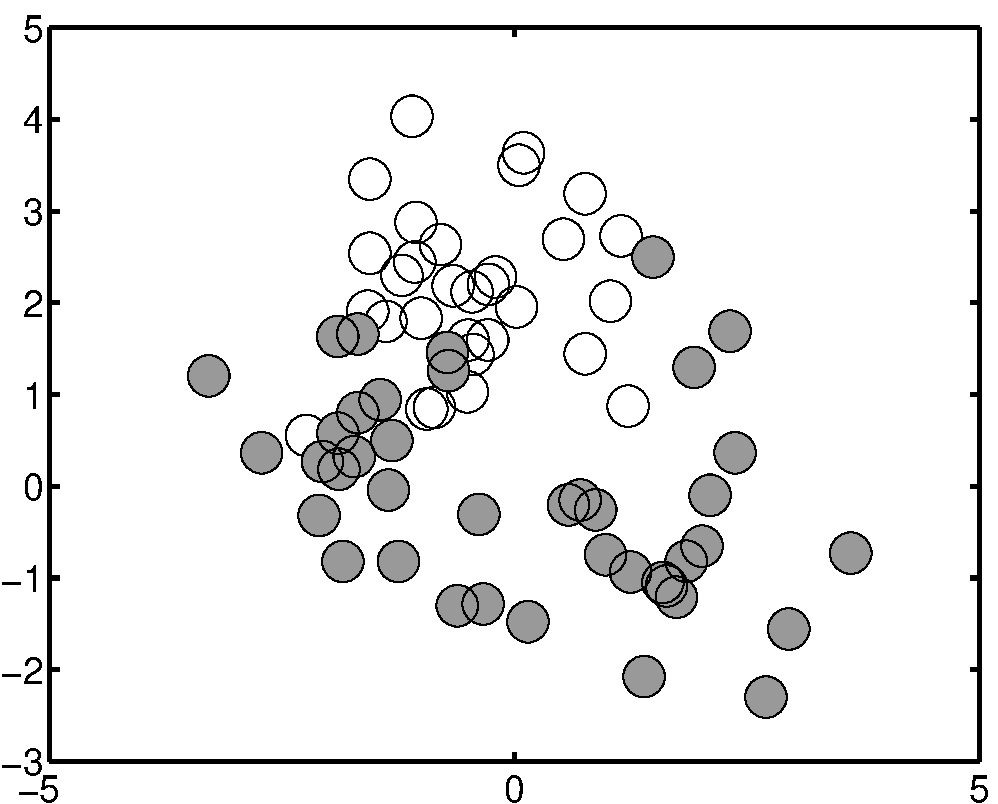
\includegraphics[width=0.7\linewidth]{class_data.pdf}
		\centering\caption{\label{fig:class_data}Some simple classification data}
	\end{figure}
\end{frame}

\begin{frame}
	\frametitle{Example - binary classification}
	\begin{figure}[tbh]
		\centering\includegraphics<1>[width=0.75\linewidth]{gpclass_hyp1_surf.pdf}
		\centering\includegraphics<2>[width=0.75\linewidth]{gpclass_hyp5_surf.pdf}
		\centering\includegraphics<3>[width=0.75\linewidth]{gpclass_hyp10_surf.pdf}
		\centering\caption{\label{fig:binary_results}Predictive probabilities averaged over 1000 Gibbs samples using an RBF covariance. As $\gamma$ is increased, the model overfits.}
	\end{figure}
\end{frame}

\begin{frame}
	\frametitle{Other things}
	\begin{itemize}
		\item Inference:
			\begin{itemize}
				\item Gibbs sampling isn't the only option
				\item A popular alternative is Variational Bayes
			\end{itemize}
		\item<2-> Ordinal Regression:
			\begin{itemize}
				\item Inference for ordinal regression follows the same process.
				\item The only difference lies in $P(y_n|z_n)$:
			\[
				P(y_n=k|z_n) = \delta(b_k<z_n<b_{k+1})
			\]
				\item Gibbs distribution for $z_n$ therefore involves a Gaussian truncated at both ends.
			\end{itemize}
	\end{itemize}
\end{frame}
